\documentclass[cn]{homework}

\title{第十五周作业}

\begin{document}
    \maketitle

    \problem
    先绘制三者的时序图如\cref{fig:trend},
    从图像上看三个序列大致都是平稳的。
    进一步做ADF检验可以知道,三个序列的$p$值皆为0.000,
    显著小于0.05,从而可以拒绝单位根的原假设,认为序列是平稳的。

    \begin{figure}[h]
        \centering
        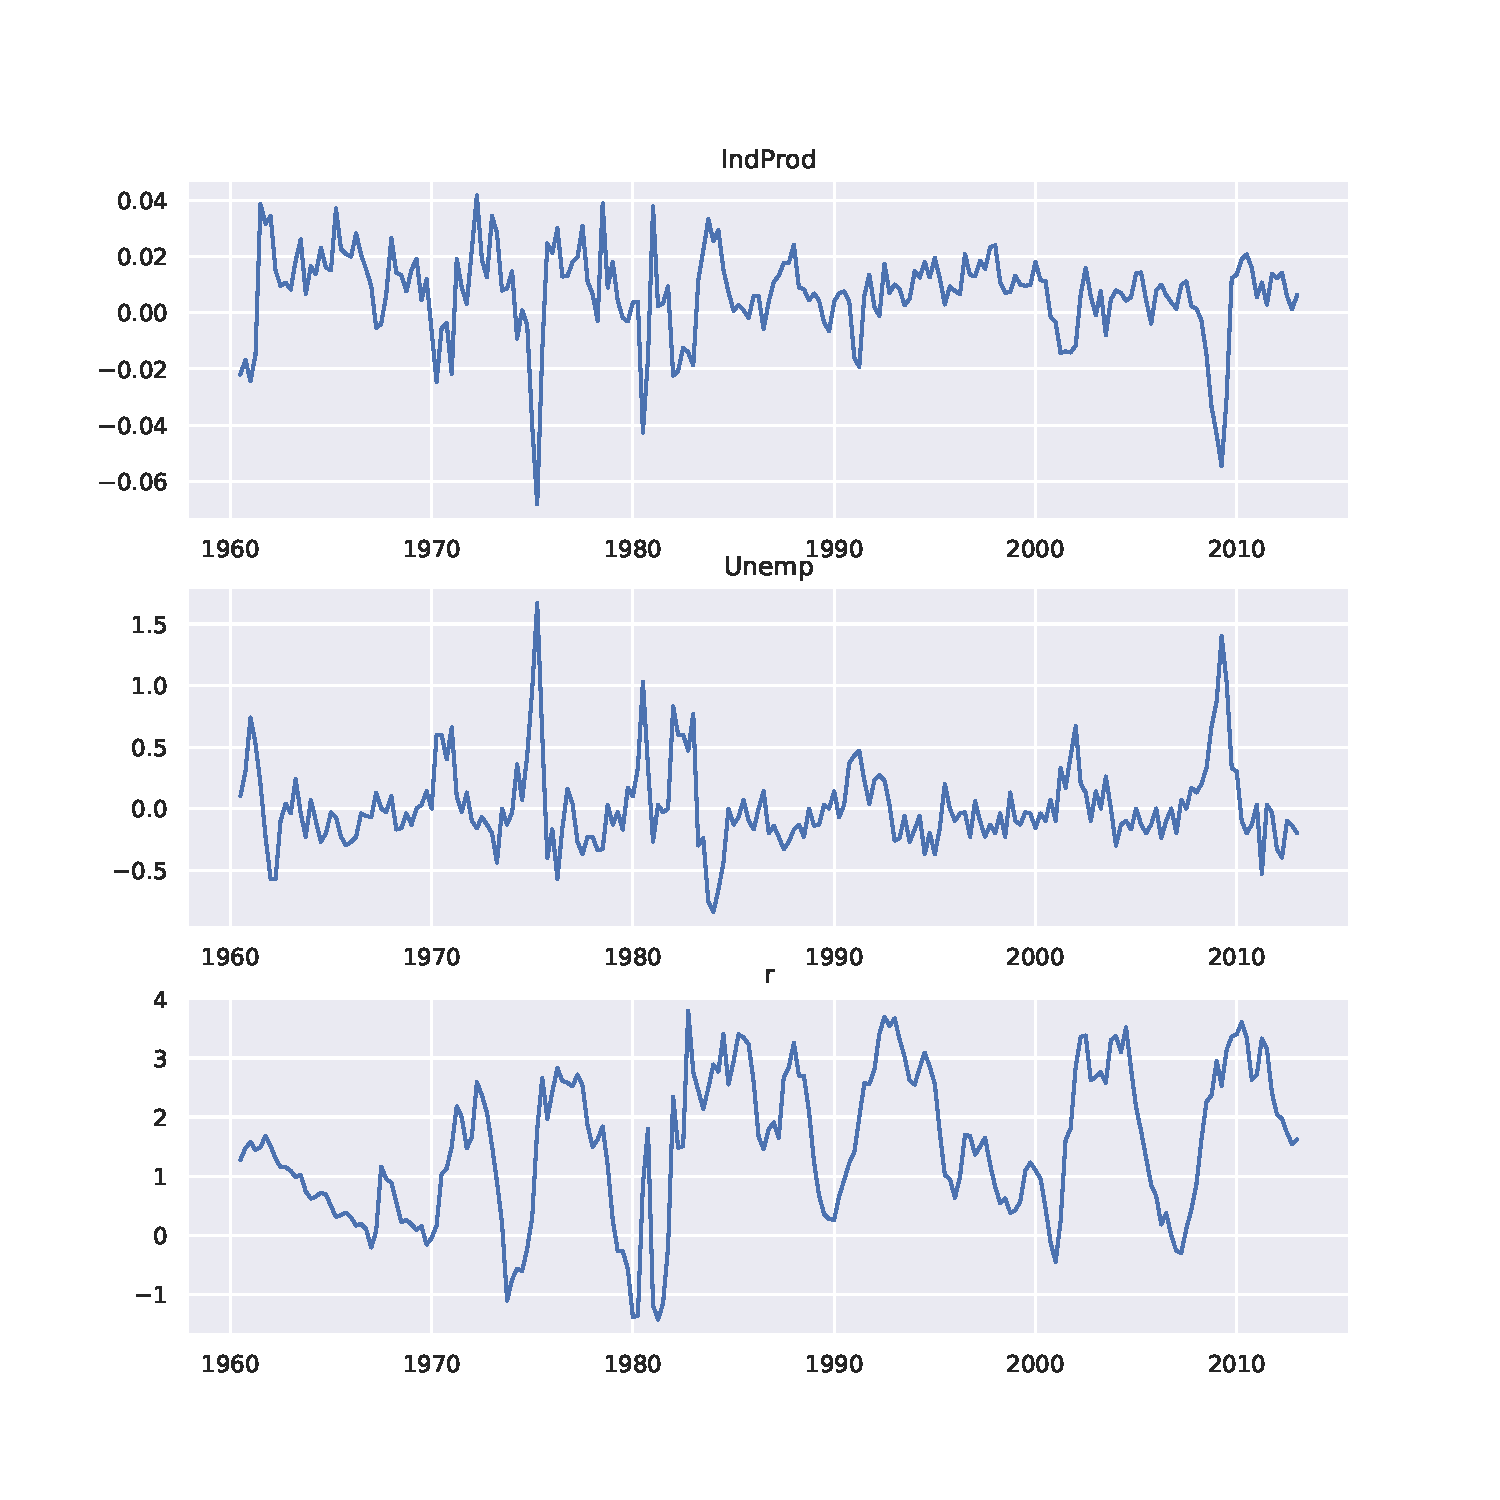
\includegraphics[width=\textwidth]{trend}
        \caption{时序图}
        \label{fig:trend}
    \end{figure}

    \begin{margintable}
        \centering
        \begin{tabular}{ccc}
            \toprule
            $p$ & AIC  & BIC \\
            \midrule
            0 & -11.098202& -11.050546\\
            1 & -13.551620& $-13.360357^*$ \\
            2 & -13.536611& -13.200779\\
            3 & -13.553569& -13.072193\\
            4 & -13.512417& -12.884513\\
            5 & -13.598659& -12.823232\\
            6 & -13.618900& -12.694941\\
            7 & $-13.661470^*$ & -12.587960\\
            \bottomrule
        \end{tabular}
        \caption{不同滞后阶数下的AIC与BIC}
        \label{tab:aic bic}
    \end{margintable}
    我们计算不同滞后阶数阶数下的AIC与BIC来合理选取滞后阶数,
    从\cref{tab:aic bic}中,AIC以$p=7$最小,BIC以$p=1$最小,
    考虑到1阶与7阶的AIC差异不是很明显,以简单的原则起见,我们
    最终决定选取滞后阶数$p=1$。于是我们可以得到拟合模型如下
    \begin{fullwidth}
    \def\ind{\text{IndProd}}
    \def\une{\text{Unemp}}
    \def\rrr{\text{r}}
    \[\begin{pmatrix}
        \ind_t\\
        \une_t\\
        \rrr_t
    \end{pmatrix}
    =\begin{pmatrix}
        0.577028 & -0.001265 & 0.001983 \\
        -3.937773 &  0.515150 & -0.006379 \\
        2.173521 & 0.555458 &  0.949893 
    \end{pmatrix}
    \begin{pmatrix}
        \ind_{t-1}\\
        \une_{t-1}\\
        \rrr_{t-1}
    \end{pmatrix}+\boldsymbol u_t\]
    \end{fullwidth}

    同时有模型的特征值为$0.4281,0.6921,0.9219$皆在单位圆内,于是模型平稳的。
    而残差的正态性检验(\cref{tab:normality})表明残差是正态的,
    \begin{table}
        \centering
        \begin{tabular}{ccc}
            \toprule
            统计量 & 临界值 & p值 \\
            \midrule
            256.2 & 12.59 & 0.000
        \end{tabular}
        \caption{残差正态性检验}
        \label{tab:normality}
    \end{table}

    考虑其中一个变量被另外两个变量解释的格兰杰因果检验(\cref{tab:Granger}),
    可以看出变量之间都具有很强的因果关系。
    \begin{table}
        \centering
        \begin{tabular}{lccc}
            \toprule
            被解释变量 & $F$统计量 & 临界值 & p值 \\
            \midrule
            r & 9.211 & 3.010 &  0.000 \\
            IndProd & 65.60 & 3.010 & 0.000 \\
            Unemp & 59.51 & 2.619 & 0.000 \\
            \bottomrule
        \end{tabular}
        \caption{格兰杰因果检验}
        \label{tab:Granger}
    \end{table}

    最后得到10期脉冲响应函数图像如\cref{fig:irf},
    以Unemp为例,可以看出在开始一段时间内,Unemp对IndProd呈现负的影响,
    但长期趋势是正的影响;Unemp对利率差r呈现正的影响,并在3、4期左右达到峰值。
    \begin{figure}[h]
        \centering
        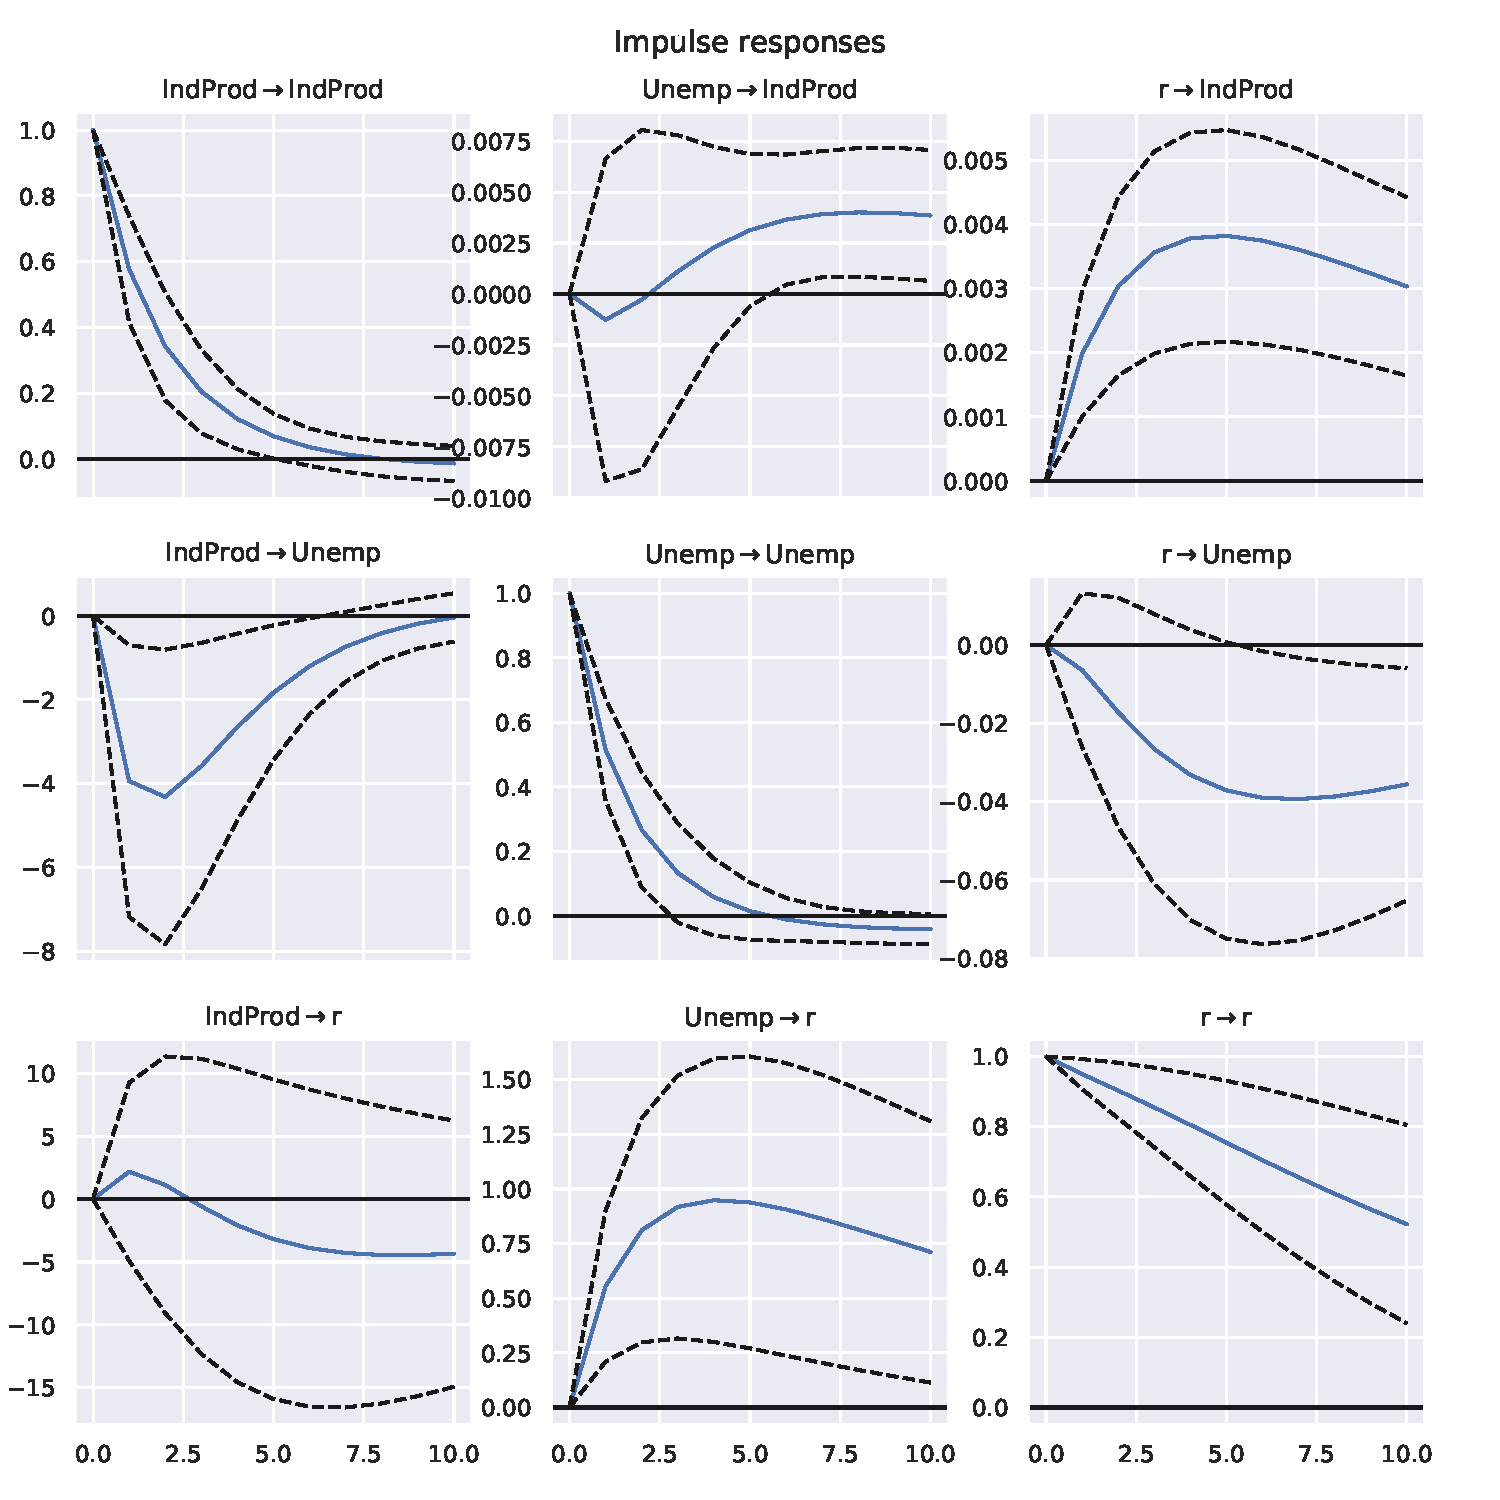
\includegraphics[width=\textwidth]{irf}
        \caption{脉冲响应函数}
        \label{fig:irf}
    \end{figure}

    \problem
    \begin{subproblem}[(\alph*)]
        \def\by{\boldsymbol Y}
        \def\be{\boldsymbol\varepsilon}
        \item
        \begin{proof}
            考虑$\Phi$的特征值,
            有$\lambda_1=1,\lambda_2=0.8$,
            从而具有单位根,于是
            变量是$I(1)$的。
        \end{proof}

        \item
        \begin{proof}
            由于
            \[\Pi=\Phi_1-I=\begin{pmatrix}
                -0.1 & 0.1 \\
                0.1  & -0.1
            \end{pmatrix}\]
            有$\mathrm{rank}(\Pi)=1<2$,从而$\Pi\by_{t-1}$是平稳的,即
            系统中的变量具有协整关系。
        \end{proof}

        \item
        VECM形式为
        \[\Delta\by_t=\begin{pmatrix}
            -0.1 & 0.1 \\
            0.1  & -0.1
        \end{pmatrix}\by_{t-1}
        +\be_t\]
    \end{subproblem}

    \appendix
    \section{代码(Python)}
    \lstinputlisting[language=R]{var.py}
\end{document}